\begin{figure}
	\begin{center}
		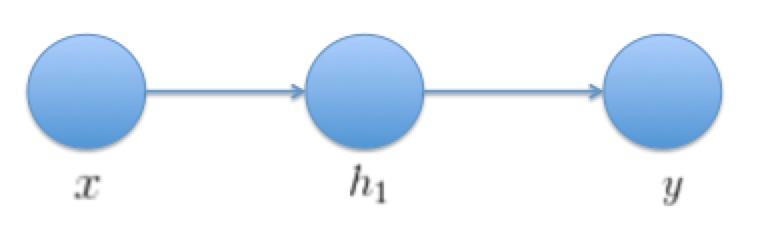
\includegraphics[width=0.35\columnwidth]{regression.png}
	\end{center}
	%\begin{center}
	%	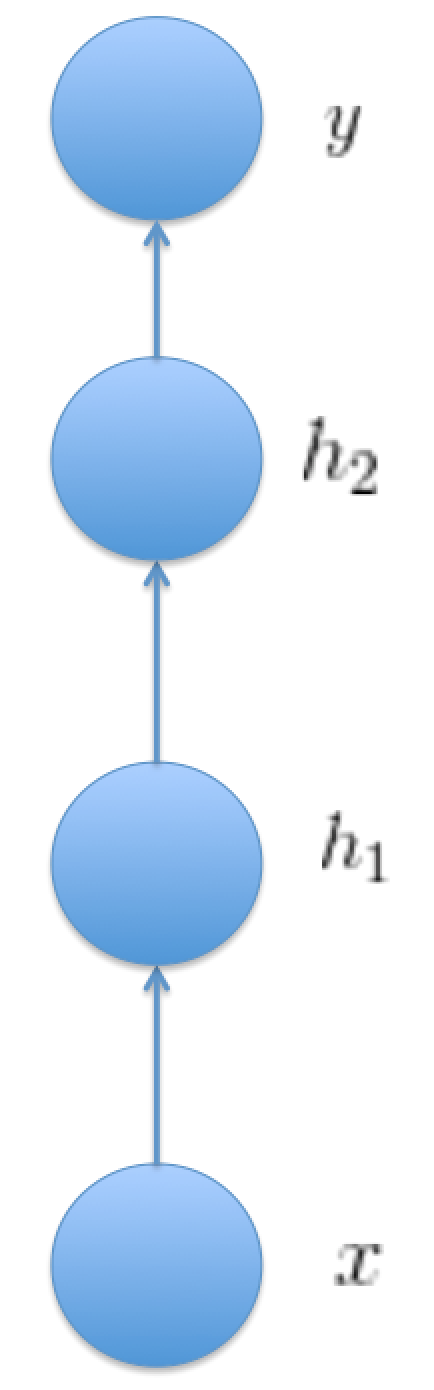
\includegraphics[width=0.3\columnwidth]{xor.png}\hspace{+0.5mm}
	%	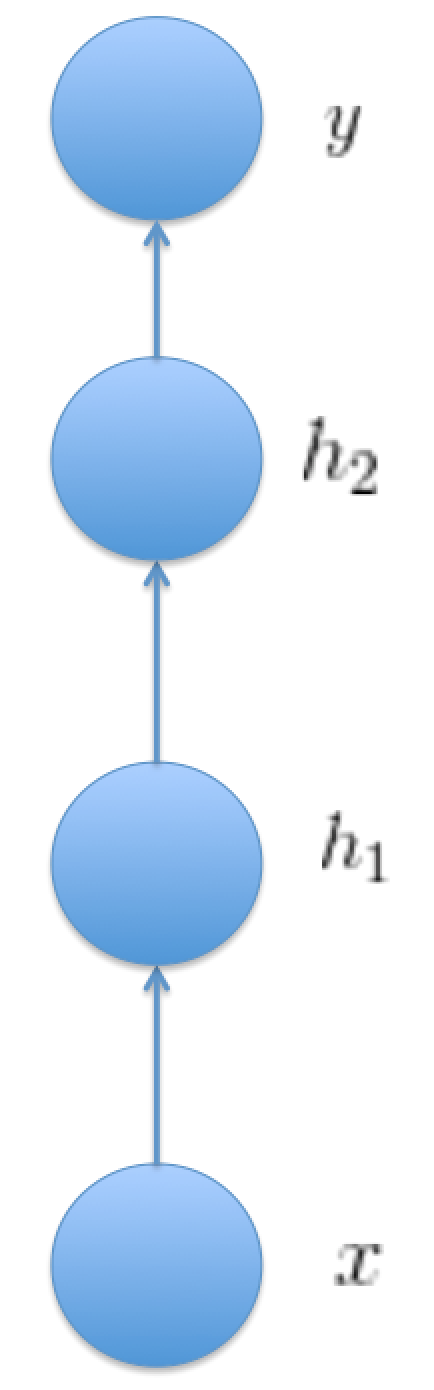
\includegraphics[width=0.3\columnwidth]{xor.png}\vspace{+1mm}\\
	%\end{center}
	%\hspace{+0mm}
	%\vspace{-2mm}
	\caption{Case 2: a comprehensive study of a two-layer linear neural network for regression task. We minimize the $L_2$ distance between the prediction $\hat{y}=W_2(W_1\mathbf{x}+\mathbf{b}_1)+\mathbf{b}_2$ and $y$. The latent representation $\mathbf{h}=W_1\mathbf{x}+b_1$ is a linear mapping.}
	\label{fig-regression}
\end{figure}
\subsection{Case Study 2: a Comprehensive Analysis on a Regression Problem}
Next, we analyze a two-layer linear neural network as shown in Figure \ref{fig-regression}. Denoting the input as $X=[\mathbf{x}_1,\mathbf{x}_2,...]$ and the target as $Y=[\mathbf{y}_1,\mathbf{y}_2,...]$. The regression loss can be formulated as:
\begin{eqnarray*}
\mathbf{E}\{||y-W_2W_1x||^2\} 
\end{eqnarray*}
where the latent feature is $\mathbf{h}=\phi(\mathbf{x})=W_1\mathbf{x}$. The optimization of $\{W_1,W_2\}$ in this multi-layer linear neural network is not trivial, since it satisfies following properties:
\begin{enumerate}
\item The regression loss is non-convex and non-concave. It is convex on $W_1$ (or $W_2$) when the other parameter $W_2$ (or $W_1$) is fixed, but not convex on both simultaneously;
\item Every local minimum is a global minimum;
\item Every critical point that is not a global minimum is a saddle point;
\item If $W_2*W_1$ is full-rank, the Hessian at any saddle point has at least one negative eigenvalue.
\end{enumerate}
We refer interested readers to \cite{nn-global-minima,deep-global-minima} for detailed analysis. 

In case of the uniform $L_2$ feature penalty, the problem becomes:
\begin{equation}
E(W_1,W_2)=\mathbb{E}\{\frac{1}{2}||\mathbf{y}-W_2W_1\mathbf{x}||^2+\frac{\lambda_1}{2}||W_1\mathbf{x}||^2\}+\frac{\lambda_2}{2}||W_2||_F^2
\end{equation}
At the global minimum $\{W_1^*,W_2^*\}$, we should have:
\begin{eqnarray}
\frac{\partial E}{\partial W_1}|_{W_1^*}=W^T_2\Sigma_{xy}-W^T_2W_2W_1\Sigma_{xx}
+\lambda_1W_1\Sigma_{xx}=0\\
\frac{\partial E}{\partial W_2}|_{W_2^*}=\Sigma_{xy}W_1^T-W_2W_1\Sigma_{xx}W_1^T+\lambda_2W_2=0
\end{eqnarray}
where we define the variance and covariance matrix as $\Sigma_{xx}=\mathbb{E}\{\mathbf{x}\mathbf{x}^T\}$, $\Sigma_{xy}=\mathbb{E}\{\mathbf{y}\mathbf{x}^T\}$.
Carrying out $Eqn(7)*W_1^T-W_2^T*Eqn(8)=0$ reveals a very interesting conclusion:
\begin{equation}
\lambda_1\mathbb{E}\{||W_1\mathbf{x}||^2\}=\lambda_2||W_2||_F^2
\label{eqn:equal-energy}
\end{equation}
This reads as \textit{\textbf{the expected $L_2$ feature penalty should be equal to final-layer weight regularizer when converged}}. Or equivalently, when close to convergence, the $L_2$ feature penalty reduces over-fitting by implicitly penalizing the corresponding weight matrix $W$. A more generalized form is:
\newtheorem{theorem}{Lemma}
\begin{theorem}
For a cost function of form in Eqn (\ref{eqn:final-cost}) with uniform $L_2$ feature regularization:
\begin{eqnarray*}
\arg\min_{W,\phi}\mathbb{E}\{l(W,\phi(\mathbf{x}^i),y^i)+\lambda_1||\phi(x_i))||^2\}+\lambda_2||W||_F^2
\end{eqnarray*}
we have:
\begin{equation}
\lambda_1\mathbb{E}\{||\phi(\mathbf{x})||^2\}=\lambda_2||W||_F^2
\end{equation}
\end{theorem}
The $\phi(.)$ can take a quite general form of a convolutional neural network with many common non-linear operations such as the ReLU, max-pooling and so on. One can follow the derivation of Eqn(\ref{eqn:equal-energy}) to easily derive \textbf{Lemma 1}.

Lemma 1 also reveals the importance of adding the weight penalty $||W||^2_F$ in Eqn(\ref{eqn:final-cost}). If we only include the the feature penalty and drop the weight penalty ($\lambda_2=0$ in our case), then a scaling as $\phi(.)=\gamma\phi(.)$ and $W=\frac{1}{\gamma}W$ with $\gamma<1$ will always decrease the energy and the solution will become very ill-conditioned with $\gamma\rightarrow 0$.